\chapter{Evaluation} % ~ 10 pages
\label{chap:evaluation}
This chapter presents and evaluates the simulation output of all the investigations that were performed with the model of the hippocampus \cite{HippSimModel.1} \cite{HippSimModel.2}. First elaborating on the initial work, with the synthetic input, before a short overview of the output analysis and its relevance is supplied. After that, the most extensive analysis is performed on the attack-related simulations. 


\section{Simulation Input}
    This section is concerned with the different versions of model input, that were used throughout this work. That includes the synthetic input, that was created and used in the beginning, as well as EEG files that later were used as its alternative.\\
    The synthetic input was developed and evaluated with the first version of the model code \cite{HippSimModel.1}. Therefore, the output analysis and reference results were derived from the paper associated with the same model version \cite{Aussel.2018}, ensuring the best possible comparability.\\
    These reference values will be presented before more details about the synthetic input and its alternative are discussed. 


    \subsection{Reference Output Values}
    % Estabilish baseline (sollparameter)
        % values of paper
            % LFP Plots during sleep
            % Event parameters (Sharp wave ripples)
                % values they derived with realistic 
    Before the simulation output can be interpreted and properly evaluated, it is necessary to elaborate on the analyzed aspects and present the reference values that were considered to be realistic. Generally, the input was assumed to be better, the more similar its output was to the values, that were derived from the original works of \textcite{Aussel.2018} (see Figure \ref{fig:input_reference}).
    
    \begin{figure}
        \centering
        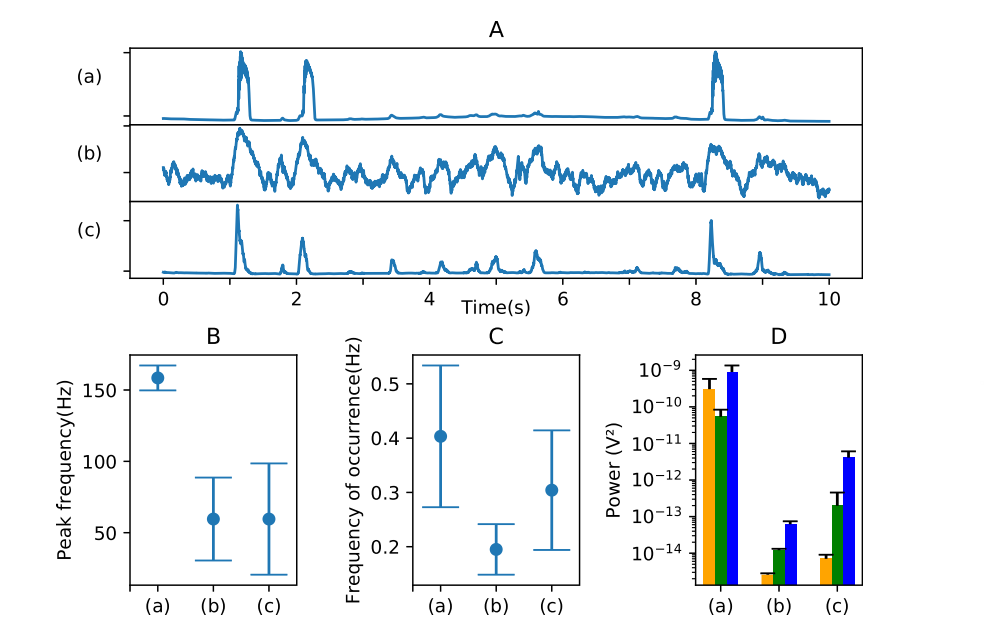
\includegraphics[width=1\linewidth]{images/Sleep Input reference Figure Aussel.2018.png}
        \caption{Main reference graphs derived from \textcite{Aussel.2018}, showing the model behavior during sleep in different network settings. Values of \textbf{(a)} were considered for the evaluation of the input, as they were produced in the realistic network configuration, employed by this work. The other values represent the model behavior in a less realistic connectivity \textbf{(b)} or topology \textbf{(c)} setting. \textbf{A:} LFP signal, plotted over time. \textbf{B:} Peak frequency of detected events. \textbf{C:} Event occurrence frequency. \textbf{D:} Power in the ripple (120-200Hz, yellow), gamma (30-100Hz, green), and theta (5-10Hz, blue) oscillation frequency bands.}
        \label{fig:input_reference}
    \end{figure}
    
    The most fundamental output analysis was performed on the raw \textbf{LFP} time series, constituting the unprocessed simulation output. The values of these files represent voltages recorded with a sampling frequency of 1024Hz \cite{HippSimModel.1}. When plotted over time, it is possible to observe the general activity of the model. Graph \textbf{A} in figure \ref{fig:input_reference}, shows such a plot and represents the reference activity during sleep.\\
    However, more specific aspects of the model output need to be observed, to evaluate cognitive processes like memory formation. In this context, the investigation of certain activity patterns was performed, as presented in more detail in the design section. Specifically sharp wave ripples, consisting of a sharp wave (also labeled as events) with superimposed ripple oscillations (100-250Hz), could be related to the cognitive process.\\
    The strongest oscillation frequencies during a detected event (also labeled as "\textbf{peak frequency}"), therefore represent an important aspect of the simulation output. The reference values for this parameter, lie approximately between 150 and 165 Hz, as graph \textbf{B} of figure \ref{fig:input_reference} indicates.\\
    Since SWRs, fundamentally rely on the occurrence of \textbf{events}, their general occurrence frequency is of central importance as well. Based on graph \textbf{C}, this work considered values between 0.3 and 0.5Hz as realistic, translating into 18-30 events per minute.\\
    Lastly, the power spectrum of detected events was also analyzed in a more general way. By deriving the mean power of the ripple, gamma, and theta frequency bands, the overall power distribution can be observed. A realistic distribution is shown in graph \textbf{D} of figure \ref{fig:input_reference}, where the ripple and theta bands, carry more power than the gamma band.

        

    \subsection{Synthetically Produced Output}
    With the input generation function, presented in the implementation chapter, a series of parameter values were explored. Specifically, the influence of frequency, amplitude, and wave realization interval on the model behavior was investigated. First, the most relevant observations concerning every parameter will be shown and discussed, before the most realistic parameter value combination is identified and evaluated. After that, some important implications of these findings on SWRs and their properties will be summarized. 
    

        \subsubsection{Parameter Analysis}
        % Amplitude 
            % no significant influence due to normalization
        Evaluating the importance of every parameter, it quickly became apparent, that the \textbf{amplitude} parameter \(A_1\), did not have any significant impact on the simulation results. This could be attributed to the way that the input equation was implemented. Specifically, in the process of translating the amplitude values into Frequencies, their magnitude is lost through normalization. Whilst this was done to ensure a maximum value for the stimulation frequency of 200Hz, it rendered the parameter useless. Nonetheless, all further investigations were performed with a uniform amplitude value of 1.
        
        % frequency influence
            % two extreme examples (F5, F1, F0.1) -> LFP graphs
                % scales event occurence
                % no more power and events at to high value
        Running the simulation with a series of \textbf{frequency} values, revealed a strong relationship between the generated input and resulting LFP values. This can be well observed in figure \ref{fig:input-LFP-comp-0.1_5}, comparing the LFP plots of two simulations with different frequency values. Whilst some activity deviates from the square wave pattern, the general shape can still be recognized. The activation phases further seem to be occurring at the same (or very similar) frequency as specified by \(f_1\).\\
        \begin{figure}[htbp]
            \centering
            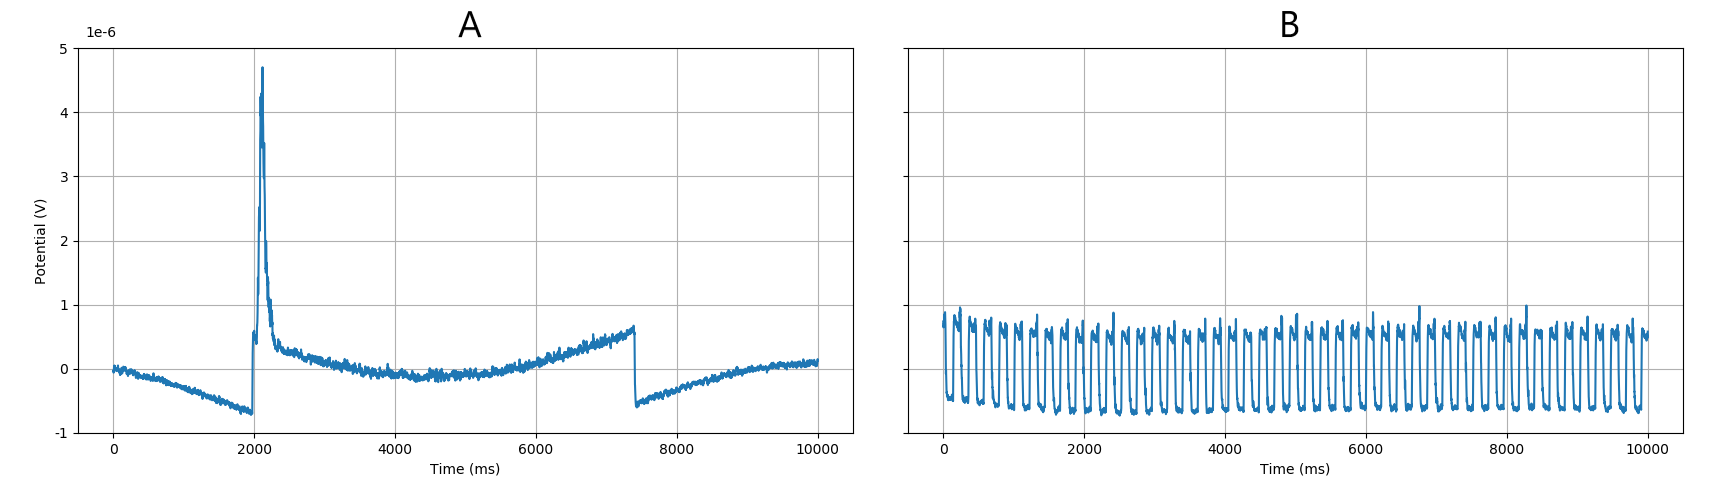
\includegraphics[width=1\linewidth]{images/Input_LFP_f01-5_labeled_only.png}
            \caption{Comparison of two 10-second LFP traces, with different input frequencies. Illustrating the impact and relevance of parameter \(f_1\), by employing fixed values for the remaining parameters (\(A_1 = 1, w = 1\)). \textbf{A:} \(f_1 = 0.1Hz\). \textbf{B:} \(f_1 = 5Hz\)}
            \label{fig:input-LFP-comp-0.1_5}
        \end{figure}
        A similar observation was made regarding the event occurrence, which correlates strongly with the number of activation phases and therefore also with the input frequency. However, it was found that if the frequency was too high, almost no more events were detected. For example during simulation \textbf{B}, figure \ref{fig:input-LFP-comp-0.1_5} (configured with an input frequency of 5Hz), events only occurred at the beginning and end of the simulation, but not during the high-frequency stimulation phase. The few events that occurred further showed poor peak frequency values (with a mean of 16Hz) and carried almost no power in all three, but especially the ripple frequency band.
        
        % wave realization interval
            % Example: F=1, A=1 with W=1,2,3,4
            % influence mostly on event occurence -> plot depending on W
                % also large jump in power and frequency from 1-2 later more stable
                % allows for higher power and peak frequency through pause
        Initial explorations of the \textbf{wave realization interval} (\(w\)) parameter, were performed with fixed values for the input frequency and amplitude (\(f_1 = 1, A_1 = 1\)). Like this, the effects of the parameter were isolated, revealing a large impact on all the aspects presented in the previous section.\\
        \begin{figure}[htbp]
            \centering
            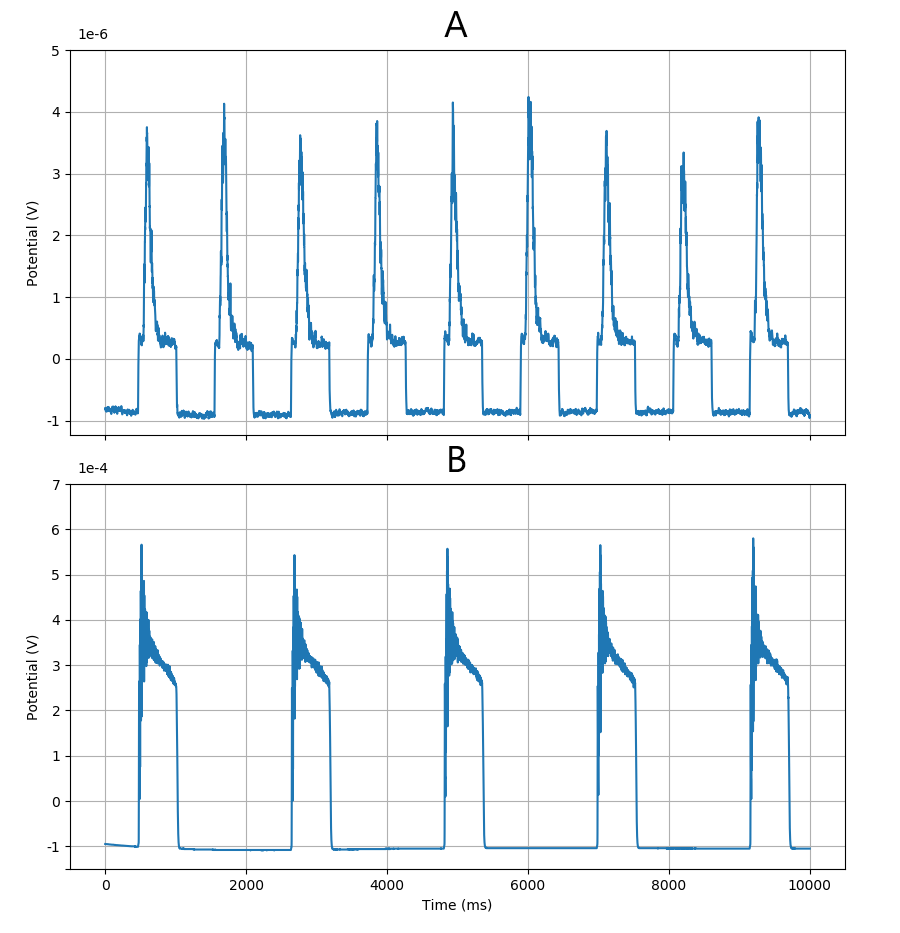
\includegraphics[width=0.5\linewidth]{images/lfpComp1-2.png}
            \caption{Two 10-second LFP traces, representing the isolated influence of the wave realization interval \(w\), with remaining parameter values of (\(A_1 = 1, f_1 = 1\)). \textbf{A:} \(w = 1\), not affecting the base input. \textbf{B:} \(w = 2\), realizing only every second input wave.}
            \label{fig:lfp_wave_int}
        \end{figure}
        
        Coinciding with the observations made in the context of the input frequency, the LFP traces reflect the input values very closely. As illustrated in figure \ref{fig:lfp_wave_int}, the reduction of input waves is directly translated into the same reduction of activity phases, measured in the LFP signal. However, the LFP plots already indicate a larger impact of the parameter. Increasing \textit{w} from 1 to 2 not only changed the shape of detected waves but also increased their amplitude.\\
        Further changes were observed in output aspects, related to SWRs. Figure \ref{fig:input_w_events} illustrates the development of event occurrences (\textbf{A}), their peak frequencies (\textbf{B}), and power bands (\textbf{C}) for \(w: [1, 4]\).
        
        \begin{figure}[htbp]
            \centering
            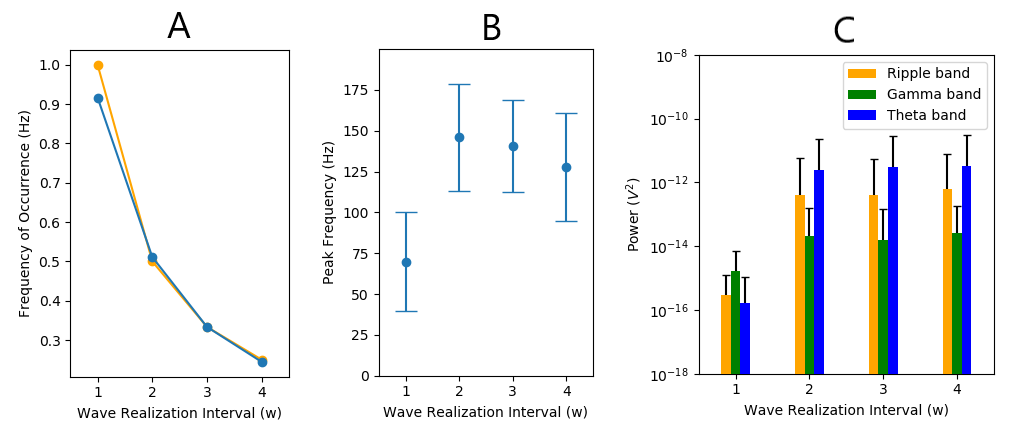
\includegraphics[width=1\linewidth]{images/input_w_labeled_event_plots.png}
            \caption{The impact of the wave realization parameter on the most important aspects of events. All data was collected from simulations with remaining input parameters: \{\(A_1 = 1, f_1 = 1\)\}. \textbf{A:} Shows the detected event occurrence frequency in \textit{blue}, compared to the frequency of realized input waves in \textit{orange}. \textbf{B:} Mean and standard deviation, of the highest power frequencies in detected events. \textbf{C:} The power of ripple (120-200Hz), gamma (30-100Hz), and theta (5-10Hz) frequency bands in detected events. Following the frequency ranges defined by the reference paper \cite{Aussel.2018}.}
            \label{fig:input_w_events}
        \end{figure}
        The event occurrence frequency is the parameter that changes most consistently with the value of \textit{w}. Plot \textbf{A} of figure \ref{fig:input_w_events} illustrates this continuous decrease, whilst also comparing it to the frequency of realized input waves. It can be observed that these two frequencies scale almost identically with the increasing values for \textit{w}. This aligns very well with the previous observations, indicating a strong coupling between the input waves, measured LFP activity phases, and the occurrence of detectable events.\\
        The other two graphs of figure \ref{fig:input_w_events} however, seem to show a different and less consistent effect of \textit{w} on events. One that is very similar to what was observed with the LFP amplitude, where the strongest changes happen between values 1 and 2. Whilst this step leads to the appearance of way more realistic values for both peak frequency and general power values, it does not scale with larger parameter values.\\
        These observations could for example be explained by a certain time threshold between these phases that must be reached before the network can produce a sufficiently strong activity event again. Such a necessity for refractory periods could further explain the observation,  that events cease to appear when the input frequency is too high.\\
        It was however not possible to explore more details regarding this effect, like specific threshold values, in the context and scale of this work.



        \subsubsection{Derived Input Parameter Combination}
        % Best result: F=1.5, A=1, wr=4
            % show stats
            % evaluate
        Throughout the exploration of the parameter space, it was possible to identify a combination of them, which yields \textbf{realistic values} for most aspects of the simulation output. Specifically by generating the sleep input with \textit{Amplitude} \(A_1 = 1\), \textit{input frequency} \(f_1 = 1.5\) and \textit{wave realization interval} \(w = 4\), the reference output values shown in figure \ref{fig:input_reference} could mostly be reproduced.
        \begin{figure}[htbp]
            \centering
            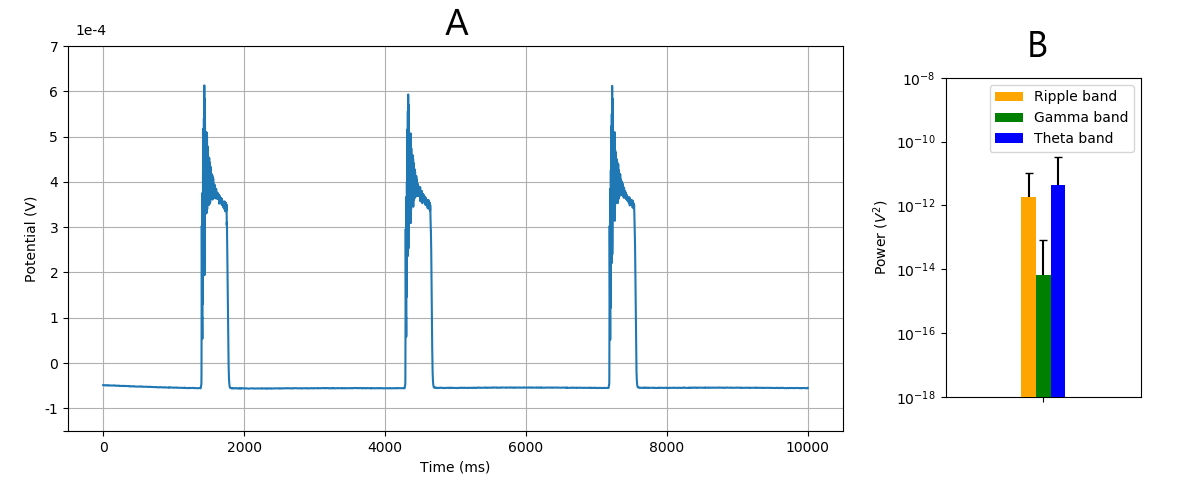
\includegraphics[width=1\linewidth]{images/BestLFPBands.png}
            \caption{Output generated with best parameter combination identified. \textbf{A:} 10-second LFP trace. \textbf{B:} Power in oscillation frequency bands (ripple (120-200Hz), gamma (30-100Hz), and theta (5-10Hz)).}
            \label{fig:best-input-plots}
        \end{figure}
        Resulting in the LFP plot and power bands of figure \ref{fig:best-input-plots}, which are quite similar to the reference regarding shape and power distribution. However, the power amplitude of all frequency bands is a bit lower than documented by \textcite{Aussel.2018}. The remaining event-related output aspects amounted to the following values:
        \begin{itemize}
            \item \textbf{Frequency of occurence}: 0.35Hz, or 21 events per minute, are very close to the mean value
            \item \textbf{Peak frequency}: 167Hz, which is just at the upper limit of the reference standard deviation, but within the bounds of all encountered ripple frequency band definitions.
        \end{itemize}
        Whilst all the reference values could be mostly reproduced with the above-presented input parameters, this synthetic input should not be considered a completely realistic alternative to EEG files. Especially since the presented reference values are only a collection of relevant, but not all output aspects. For example, the duration of detected events was not considered and unfortunately cannot be reproduced realistically with this input.
        
            
        \subsubsection{Implications on Sharp Wave Ripple Stimulation}
        % events occur with strong input injection
            % which by default and implementation details represents synchronus activation of many neurons
                % triggers 
        % high enough power and peak frequency only when
            % breaks long enough
            % than seem to scale with f
        The exploration of different input parameters showed some interesting correlations between input and SWRs. This section aims to summarize and evaluate these findings since they may guide the development of a countermeasure approach, based on brain-computer interfaces.
        
        In general, many findings showed a strong correlation between a large area stimulation of the entorhinal cortex by the input, the resulting LFP measurements, and the emergence of SWRs. This potential connection between brain stimulations and SWRs was however observed when the input was injected via the simulation of frequencies and not by currents. Implications on current injections that would be performed by BCIs are therefore limited.\\
        The second observation was that sufficiently strong events, with suitable oscillation frequencies, only occurred with long enough time intervals between them. This phenomenon might not only be restricted to frequency stimulation and should therefore also be considered in the context of brain-computer interfaces and current injections. 

            
        
    \subsection{Comparison to EEG Input}
    % own eeg file sim doesn't produce realistic ouput with their analysis function
        % may be different to the ones used in Aussel.2018
    % general differences and pros/cons observed
        % way more consistant and controllable "base case"
        % stereotypical behaviour of synthetic input
            % strong coupling to output
        % implications on real brain questionabel
            % due to big difference
    Exploring a synthetic input not only allowed for the exploration of its effects on SWRs but also enabled a comparison to EEG files. This shall provide an overview of both options and evaluate their suitability for different brain simulation contexts.\\
    Simulations that were performed with the later received EEG files, yielded LFP measurements that were completely unlike anything \textcite{Aussel.2018} presented as simulation output in this primary paper (see figure \ref{fig:EEG-LFP}). Even though they were performed using the same model code. Lacking any other indications, this is attributed to the fact that the received EEG files stem from later research and may differ from what was used in the reference paper.
    \begin{figure}[htbp]
        \centering
        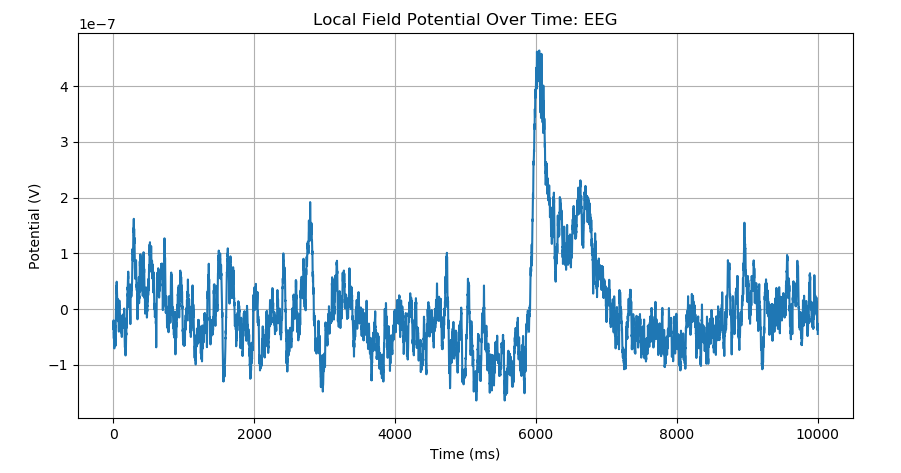
\includegraphics[width=0.75\linewidth]{images/EEG-LFP.png}
        \caption{10-second LFP trace, produced with EEG files as input.}
        \label{fig:EEG-LFP}
    \end{figure}
    Apart from the apparent differences in the LFP trace of the output, some more general observations were made in the process of working with both input types. The simulation behavior with synthetic input is for example more consistent. Resulting in smaller differences in the output values, across multiple simulations of the same configuration. This allows findings to be easier to reproduce and can reduce the amount of necessary simulations, to achieve robust mean values. This makes this option more viable if computational resources are sparse.\\
    However, the synthetic input produces rather stereotypical simulation behavior, which is strongly coupled to the specified input values. This does give a lot of control over a further parameter of the simulation but also makes related design choices extremely impactful. Consequently, a lot of research should be performed to ensure it produces realistic behavior across all relevant aspects of the simulation. Otherwise, it is questionable whether related findings have any implications on the real brain.\\ 
    By deriving the input from EEG files and therefore actual brain activity, this issue can be minimized. Making it the preferable option to perform realistic simulations and derive relevant findings. 
    


\section{Output Analysis}
% Necessary since 
% Massive impact on results
The output analysis is a core factor of the evaluations performed in this work. The values it extracts from the simulation output depend on a set of detection thresholds and frequency ranges. This section evaluates its influence on the simulation results and shows the impact of its main parameters.

% influence of peak/boundary condition
    % comparison graphic, peak distribution and duration
    % higher peak condition -> fewer false positives (shape-wise) but missing many
    % boundary condition -> strong influence on event length
    % frequency range - plot peak distribution
\begin{figure}[htbp]
    \centering
    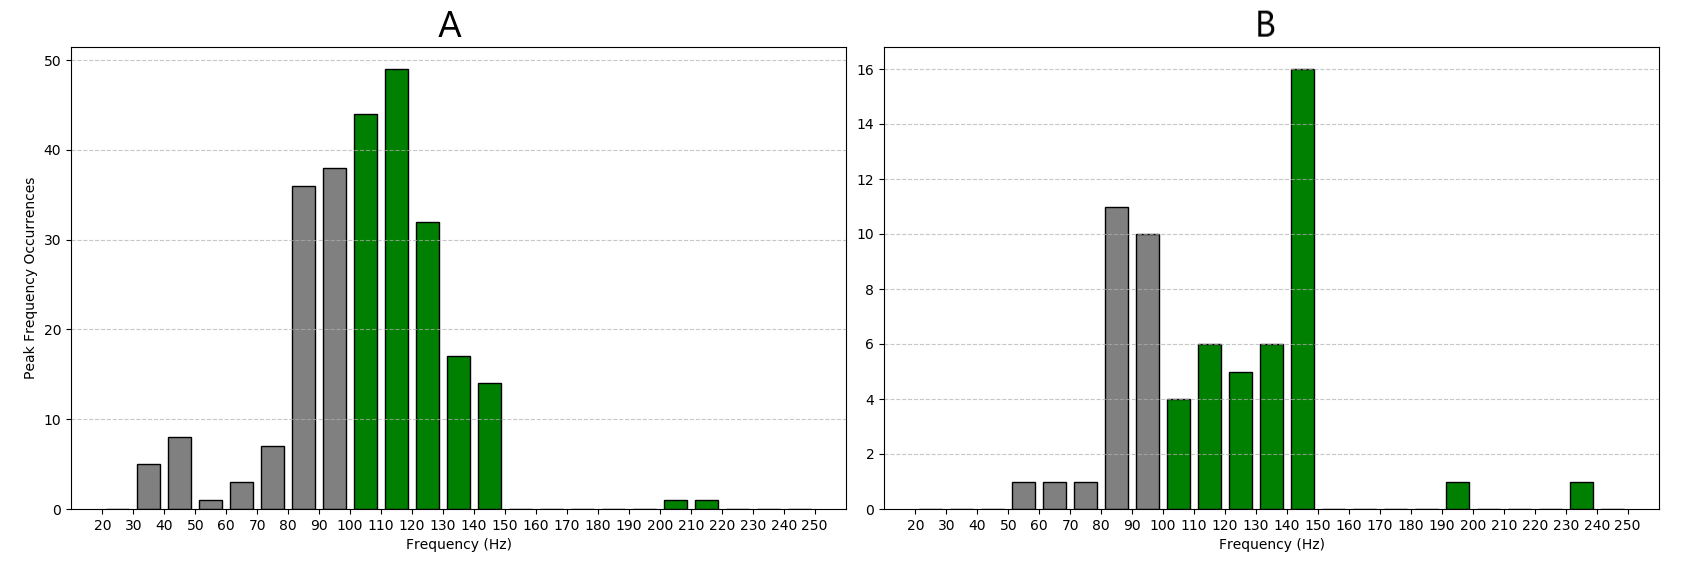
\includegraphics[width=1\linewidth]{images/Output Analysis Comparison.png}
    \caption{Event peak frequency distributions, derived from the same simulation data with different analysis parameters. Green bars represent occurrences in this work's ripple frequency range definition (100-250Hz). \textbf{A:} Derived with parameters used for remaining work (\(boundary\_condition\) = 3 x SD, \(peak\_condition\) = 4.5 x SD). \textbf{B:} Derived with boundary condition of 2 x SD and peak condition of 5.5 x SD}
    \label{fig:output_analysis_comp}
\end{figure}
A series of \textit{boundary conditions} (ranging from 2-4 x SD) and \textit{peak conditions} (ranging from 3-6 x SD) were explored in different combinations. This allowed the identification of their general influence on analysis results. This included the observation and comparison of event peak frequency distributions (like the ones depicted in figure \ref{fig:output_analysis_comp}), but also the inspection of LFP traces from detected events. The latter approach was mostly used to identify false positives (events that were detected but did not resemble a sharp wave ripple).\\
Concerning the \textbf{peak condition}, it was observed that with higher values, the ratio of false positives in detected events decreased. However, this trend was accompanied by a strong decrease in overall detected events (with almost none at a value of 6). This therefore also caused the analysis to miss many sharp wave ripples of smaller power.\\
The \textbf{boundary condition} had its strongest influence on the length of detected events. Increasing the duration of detected sharp waves, the lower its factor was chosen. Interestingly, the amount of detected events also correlated with the factor. Reaching its maximum around a factor of 3, before it decreased again with larger values.

% Why did i choose the ones I did
    % yielded realistic SWR stats in healthy condition
    % whilst not too many false positives
        % proper shape
Based on these observations, the best-suited parameters for the output analysis of this work were identified as: \(\{peak\_condition = 4.5, boundary\_condition = 3\}\). Even though these values are below the thresholds, stated to be used by \textcite{AmelieAussel.2020}, they produced the best analysis output. Yielding reasonable SWR values from healthy simulations, whilst avoiding too many false positives. Also, the results extracted with them are more robust to different definitions of the ripple frequency range, than others. This is a valuable property, considering the major differences between them.



\section{Electromagnetic Attacks}
% Effects of electromagnetic attacks on the hippocampus
    % simulating changes in the brain that are associated with rf emr
        % with a range of severities
        % comparing output to healthy baseline
    % What effects that might have on memory consolidation
% structure of section (and research approach)
    % Baseline of healthy sleep outputs
    % Mechanism-wise impact analysis (with same structure for all of them)
        % neurotransmitters, structural damage
        % The same output analysis and reference plots are provided for every scenario
            % allowing for a good comparison of parameter effects
    % Concluding with investigations of full attack (all mechanisms combined)
The core contribution of this work is to explore the underlying mechanisms of electromagnetic attacks, to establish a basis for countermeasures. Therefore, a series of brain alterations associated with RF EMR were identified and integrated into the simulation. Since the extent of alterations depends on the irradiation intensity and such values could not be identified for Neurostrikes, these alterations were explored in different severities. The resulting output was then compared to the healthy model behavior, focusing on network activities related to memory consolidation. Ultimately assessing the potential involvement of the explored mechanisms in Neurostrikes, by comparing their effects on cognition with the reported attack symptoms.\\
This section is therefore structured as follows. First, the healthy sleep activity of the model will be presented, to establish a baseline in the most important aspects. Then, two different mechanisms are investigated, based on two parameters each. Employing the same analysis structure and output representations for each simulation configuration, to facilitate their comparison. Lastly, the combination of all explored attack parameters will be evaluated in the context of a more realistic representation of Neurostrikes.

    
    \subsection{Healthy Sleep}
    % Establish a baseline of research parameters during healthy sleep
        % Necessary due to adjusted output analysis
        % Exclude any potential differences from paper reference, that could arise due to the simulation environment
    The output values presented in this section were produced with the second model version \cite{HippSimModel.2}. This model code was configured to represent a healthy sleeping configuration, and EEG files were used as input. To extract event-related data from the LFP output signal, the above-presented analysis function was employed. Doing so made it possible to establish a healthy reference value, with the exact same environment that later was used to simulate and analyze electromagnetic attacks. This ensures that potential alterations of behavior and output can solely be attributed to the attack-related parameter adjustments.\\
    In the following, the simulation results will be presented and discussed. Differentiating them also from findings made in the older model version and comparing them to relevant reference values of the model creator.

    % Plots:
        % LFP
        % Event peak frequency distribution
        % SWR Peak frequency
        % Power spectral band
    \begin{figure}[htbp]
        \centering
        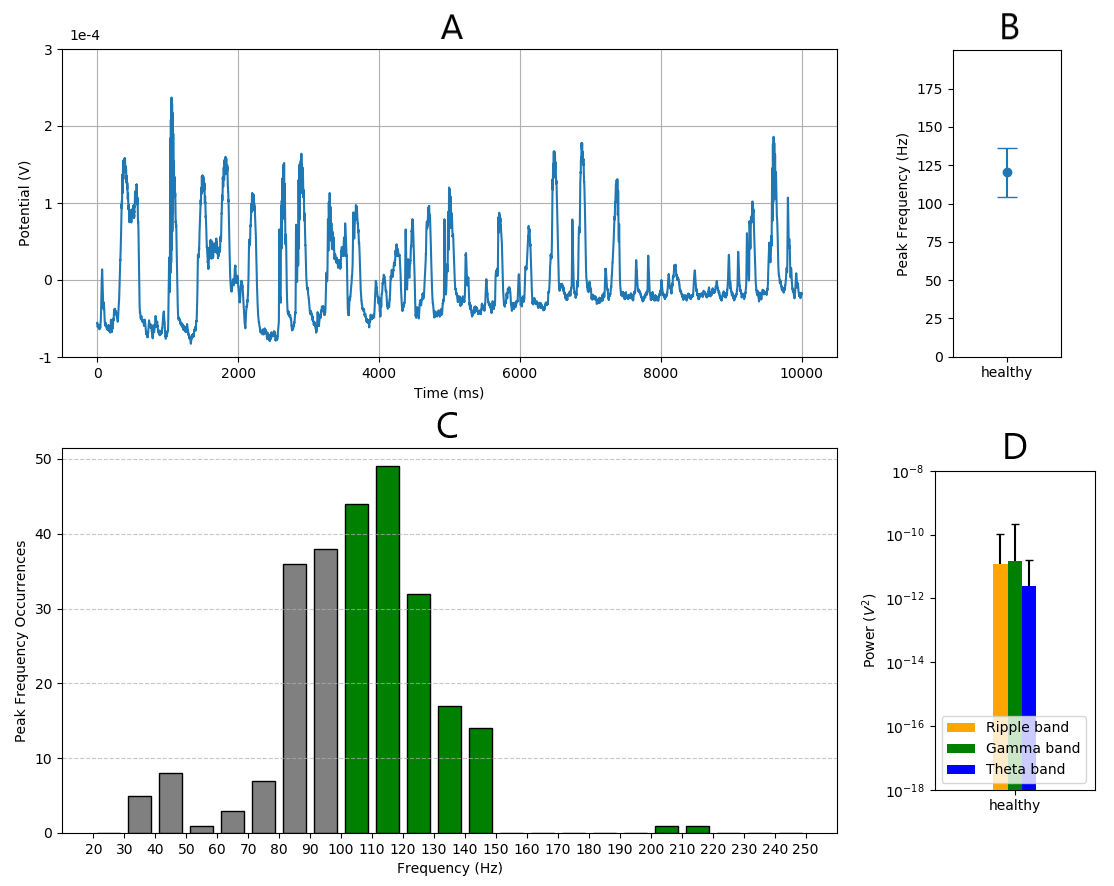
\includegraphics[width=1\linewidth]{images/attack_results/healthy_sleep_collection.png}
        \caption{Some graphical representations of the simulation output and its aspects, derived from 14 healthy sleep simulations of 60 seconds. \textbf{A:} Example of a 10-second LFP trace. \textbf{B:} Mean and standard deviation of the peak frequencies during sharp wave ripples. \textbf{C:} The distribution of peak frequencies across all detected events. Those falling in the ripple band (100-250Hz) are depicted in green and were considered sharp wave ripples. \textbf{D:} The power of detected events, analyzed in three separate frequency bands (theta: 5-10Hz, gamma: 30-100Hz, ripple: 100-250Hz).}
        \label{fig:healthy_collection}
    \end{figure}
        
    % Outputs generated on own machine
        % Short discussion of values
            % LFP different form reference for input, but way less stereotypic
            % distribution shows detected vs. selected events = swrs
        % very similar event outputs as aussel.2020
            % SWR peak freq 124 Hz vs. 125 Hz
            % SWR Occurrence 11.2 -> 0.18Hz vs. 11
        % except my events are shorter
            % SWR Duration 94 ms
            % but is consistent with swrs presented by Buszaki.2015
    The values depicted in figure \ref{fig:healthy_collection} give an overview of the general model behavior and describe the same or similar aspects, as the input reference (figure \ref{fig:input_reference}). However, the values are quite different from what the first model produced. The LFP measurements show less stereotypical behavior, and the event-related aspects differ a lot as well. Since \textcite{AmelieAussel.2020} reports very similar values with the new model version, these differences seem to be code-related.\\
    More specifically they reported a mean peak frequency of 125Hz, with a standard deviation of 20Hz, which is almost identical to the produced values shown in \textit{B}. Also, the \textbf{occurrence frequency} of 11 events per minute (~0.18Hz) aligns perfectly with the analysis results of \textbf{11.2 events per minute}. Only the sharp wave ripple \textbf{event duration}, had a significantly shorter mean value of \textbf{94ms} (compared to their reported 156ms). According to \textcite{Buzsaki.2015} however, this also lies within the bounds of realistic values.\\


    \subsection{Neurotransmitter Changes}
    % This section is concerned with Neurotransmitter changes
        % Explain
    This section evaluates the impact of electromagnetic attacks by simulating the associated changes in neurotransmitters. More precisely, the neurotransmitter acetylcholine was investigated, by adjusting two model parameters. These parameters represent the influence of acetylcholine on selected conductances in the network and reflect different levels of the neurotransmitter, depending on their values.\\
    First, each parameter was analyzed on its own, to reveal their isolated influence on the model behavior. After that, the parameters were combined to evaluate the overall effect of different acetylcholine levels on memory consolidation. 

    
        \subsubsection{Calcium Activated Nonspecific Ionchannel Conductance (gCAN)}
        % Specifying high level meaning of parameter
        % Present parameter range
            % connect with meaning (0.5 sleep concentration, 25 waking concentration)
        The parameter \textit{gCAN}, represents the conductance value of a specific ion channel, which increases with the concentration of acetylcholine. As indicated in the design section, it was analyzed across a range of values (0.5 to 25 \(\mu S/cm^2\)). The lowest value represents the healthy neurotransmitter concentration during sleep, whilst the highest value reflects a three times larger concentration.
        
        % Plot
            % describe thoroughly once
            % then reference for explanation
        \begin{figure}[htbp]
            \centering
            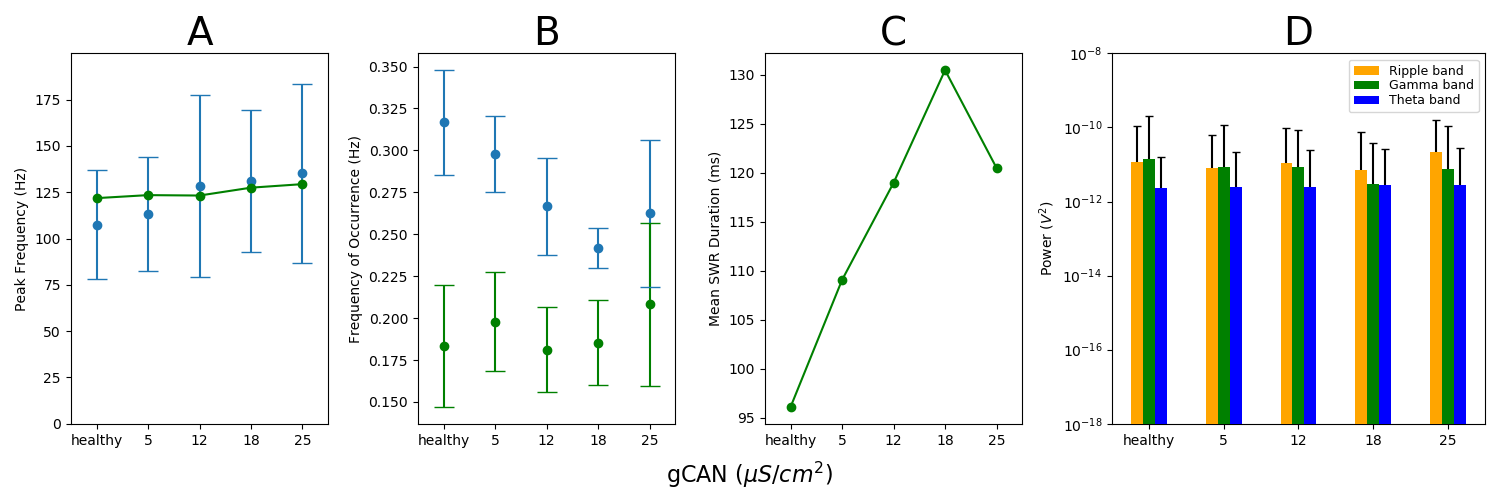
\includegraphics[width=1\linewidth]{images/attack_results/gCAN.png}
            \caption{The impact of \textbf{gCAN} on sharp wave ripples. Values across the parameter range are compared to healthy ones, regarding the most important aspects of activity patterns. To derive these results, 8 simulations of 60 seconds were performed for all depicted parameter values. \textbf{A:} Overview of peak frequencies in events. Mean and standard deviation of all events in \textit{blue}. Mean values of those qualifying as sharp wave ripples in \textit{green}. \textbf{B:} Mean and standard deviation of event occurrence frequencies. All events in \textit{blue}, sharp wave ripples in \textit{green}. \textbf{C:} Development of sharp wave ripple durations. \textbf{D:} Mean and standard deviations of the power in different frequency bands (Ripple band = 100-250Hz, Gamma band = 30-100Hz, Theta band = 5-10Hz). Calculated from all event recordings.}
            \label{fig:attack-gCAN}
        \end{figure}
        % discuss most relevant observations
        Figure \ref{fig:attack-gCAN}, shows a collection of plots, that incorporate the most important aspects of the output analysis. Allowing for a range of interesting observations. \textbf{A} indicates for example, that higher values of \textit{gCAN}, lead to an overall increase in the event peak frequency. Rising from the healthy 107Hz to a mean of 135Hz at the top of the parameter range. The largest step, however, takes place from 5 to 12 \(\mu S/cm^2\), where the mean peak already reaches 128 Hz.\\
        This increase is accompanied by an overall decrease in event occurrences (shown in \textbf{B}), although SWR are not affected by this. Their frequency of occurrence increases even. This shows that the increased peak frequency was able to overcompensate for this otherwise negative effect. At least concerning memory consolidation activities.\\
        \textbf{C} allows for the final observation of an increase in the SWR duration. But since this effect leads to a maximum duration that still lies below the values of \textcite{AmelieAussel.2020}, it was not considered an impairment of cognitive function.\\


        \subsubsection{Cholinergic Modulation of Synapse Conductances (gACh)}
        Acetylcholine also influences a series of synaptic conductances, which differ depending on the region (see the design chapter for more details). This cholinergic conductance modulation scales similarly to \textit{gCAN}, with the neurotransmitter concentration. Since the specific effects are more complex, \textit{gACh} only represents a scaling factor, which is translated into the conductance values by the model. The explored parameter range starts with 1 (representing the acetylcholine levels during sleep) and goes up to 3 (to also represent 3 times the neurotransmitter concentration).
        
        \begin{figure}[htbp]
            \centering
            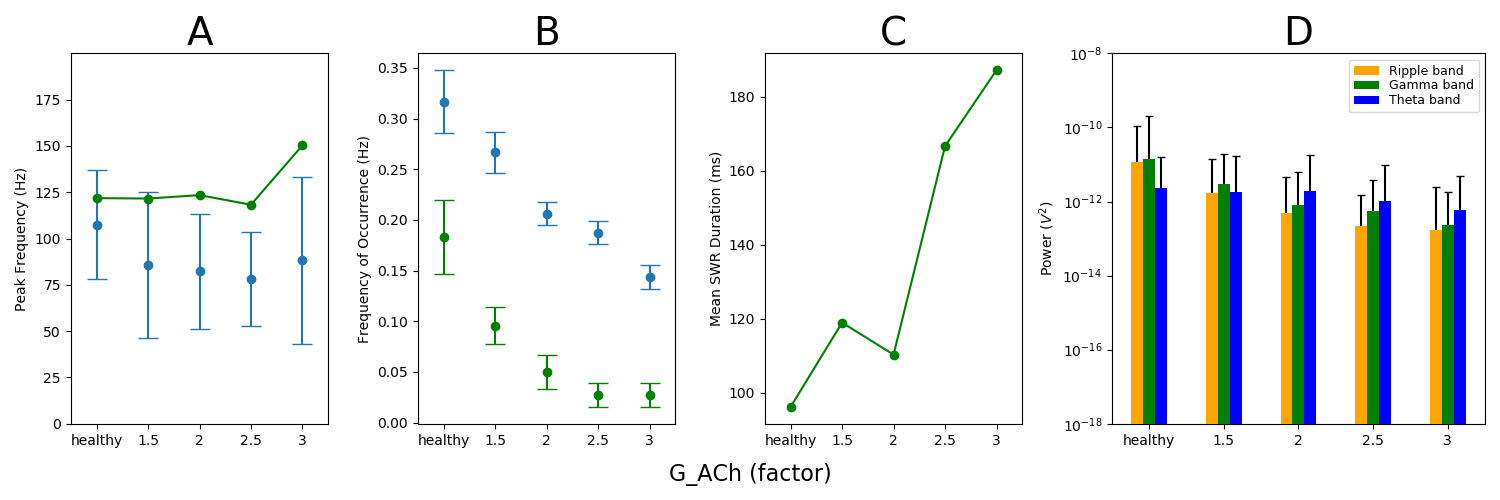
\includegraphics[width=1\linewidth]{images/attack_results/G_ACh.png}
            \caption{The impact of \textbf{gACh} on sharp wave ripples. See figure \ref{fig:attack-gCAN} for a detailed explanation. This data was derived and presented in the same fashion. Only the investigated parameter differs.}
            \label{fig:attack-gACh}
        \end{figure}
        The results presented in figure \ref{fig:attack-gACh}, indicate a notable impact of the parameter on every analyzed aspect. The general peak frequencies of events show already with the smallest increase of \textit{gACh} (to a value of 1.5), a decrease of 22Hz. Since this moves the peak values far outside the ripple frequency range, a reduction of sharp wave ripples is to be expected as a consequence.\\
        As plot \textbf{B} indicates, the reduction of sharp wave ripples, driven by the overall event decrease, indeed seems to be reinforced by this effect. During the first parameter step, the mean of all event occurrences is only reduced by about 15\%, and the number of SWRs is almost halved (from 11 to 5.75 events per minute). Beginning from a \textit{gACh} value of 2.5, the model then seems to reach a low point of SWR occurrence (0.027Hz or 1.625 events per minute). Given that sharp wave ripples play a critical role in memory consolidation \cite{Girardeau.2011}, such extreme values certainly can be associated with an impairment.\\
        Further observations show a strong increase in SWR duration, which in this case also surpasses any reference value. But also a noticeable power decrease across all oscillation bands seems to be related to an increasing value for \textit{gACh}.


        \subsubsection{Overall Effect of Acetylcholine}
        To simulate the compound effect of elevated acetylcholine levels in the hippocampus, the above-explored parameters were simultaneously adjusted. This was done by combining values that reflect a similar neurotransmitter concentration in the network. Through this, it was possible to simulate varying levels of acetylcholine in the model and observe their overall effects on memory consolidation.

        \begin{figure}[htbp]
            \centering
            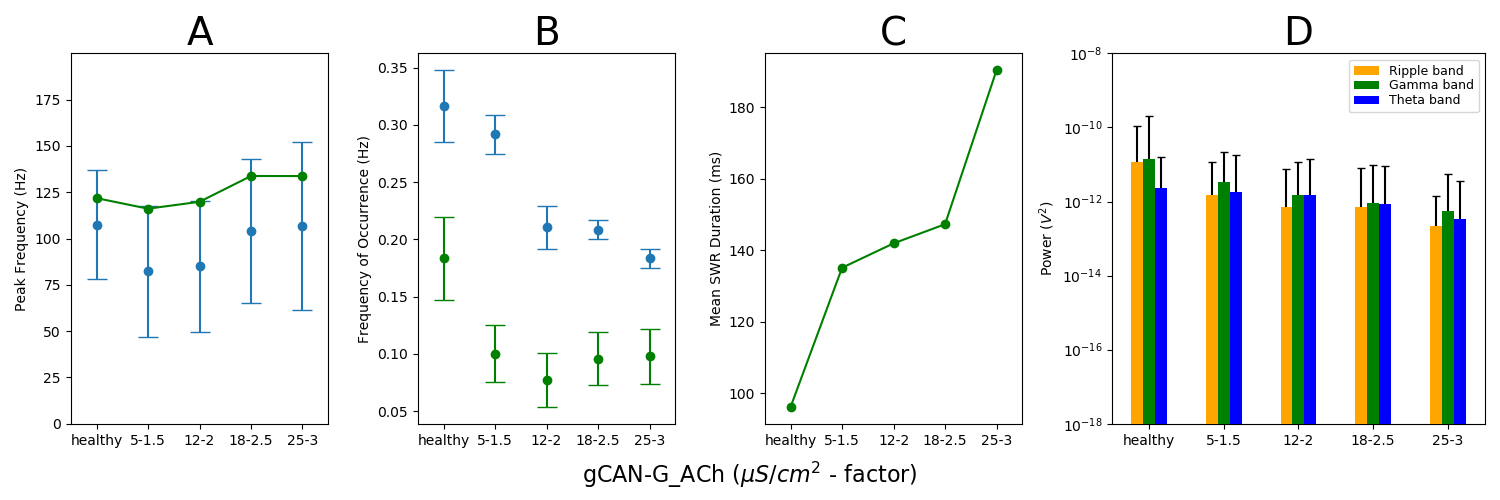
\includegraphics[width=1\linewidth]{images/attack_results/gCAN-G_ACh.png}
            \caption{The overall impact of \textbf{acetylcholine} on sharp wave ripples. See figure \ref{fig:attack-gCAN} for a detailed explanation. This data was derived and presented in the same fashion. Only the investigated parameters differ.}
            \label{fig:attack-acetylcholine}
        \end{figure}
        The combination of both parameters produced a result, in which most values lie between the ones of the individual parameters. But since the parameter \textit{gACh}, generally showed effects of larger magnitude, it tends to dominate the combined effect.\\
        This is well illustrated by the event occurrence frequencies, depicted in plot \textbf{B}. Whilst the results related to \textit{gCAN} (see figure \ref{fig:attack-gCAN}) indicated a (small) increase of SWR occurrences, the combined simulation results are way more similar to the (strong) decrease, that was shown with \textit{gACh} (see figure \ref{fig:attack-gACh}).\\
        A similar observation can be made regarding SWR durations (plot \textbf{C}) and event powers (plot \textbf{D}). Only in the aspect of event peak frequencies, where both parameters show a similar effect strength, are the results more balanced between the two influences.

        The influence of acetylcholine on memory consolidation, therefore seems to be driven by the cholinergic modulation of synaptic conductances (parameter \textit{gACh}). Overall showing a clear impact on SWRs, even at the smallest simulated deviation of the healthy sleep values. Especially the large reduction of SWR occurrences is of concern for memory consolidation. Whilst the healthy state produces 11 events in a minute, no simulated attack values allow for more than 6.\\
        Changes in acetylcholine, therefore represent a mechanism that could indeed be involved in the learning and memory impairments, reported by victims of NeuroStrikes. 
        

        
    \subsection{Structural Damage}
    % What does this section analyze
        % Electromagnetic Attack
        % by simulating a different effect of it on the network
        % Structural damage
    % How was this done
        % was represented by two parameters that reflect such damage
        % Reduction of Neurons
        % Reduction of excitatory synapse conductance
    % Mention structure of approach and section
    This section evaluates a different effect of RF EMR on the hippocampus and its implications on memory consolidation. More precisely, structural damage was simulated by adjusting parameters that reflect either neuron or synapse damage. Exploring these parameters across a range of values, allowed for their assessment in different degrees of severity.\\
    The following analysis is structured very similarly to the previous section, where both parameters are analyzed on their own before their compound effect is assessed.

    
        \subsubsection{Neuronal Damage (N)}
        % Parameter description
        Neuron damage was integrated into the model by reducing the amount of simulated neurons. This was done by adjusting the reference parameter \textit{N}, which specifies the number of neurons in a region of the network and scales the others as specified in the design section. It was explored with a healthy value of 10'000, and across a range that at its lowest value of 6'000 represents a 40\% neuron decrease.

        % Results
        \begin{figure}[htbp]
            \centering
            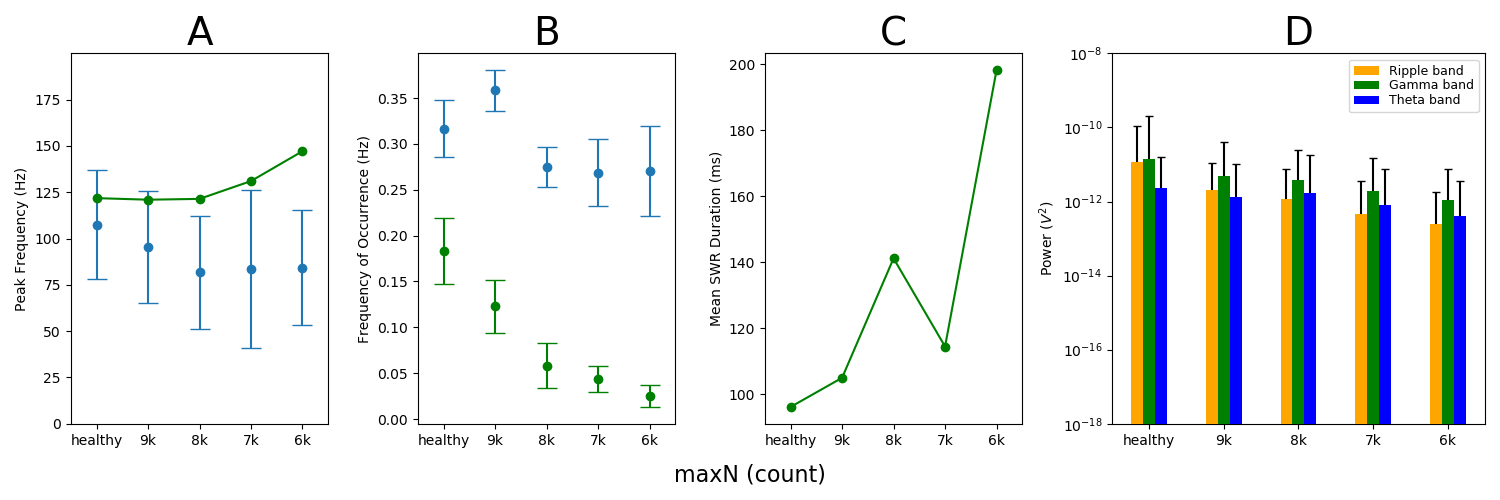
\includegraphics[width=1\linewidth]{images/attack_results/maxN.png}
            \caption{Impact of \textbf{N} on sharp wave ripples. See figure \ref{fig:attack-gCAN} for a detailed explanation. This data was derived and presented in the same fashion. Only the investigated parameter differs.}
            \label{fig:attack-neuron}
        \end{figure}
        % Evaluation of results
        The effect of a neuron reduction is relatively consistent for every step of the simulated parameter range. Ultimately resulting in severe alterations of event-related aspects.\\
        Whilst the general event occurrence remains on a similar level, the peak frequencies of the occurring events are reduced to mean values of about 80Hz. In turn, almost none of them qualify as SWRs, as plot \textbf{B} indicates.
        \begin{figure}[htbp]
            \centering
            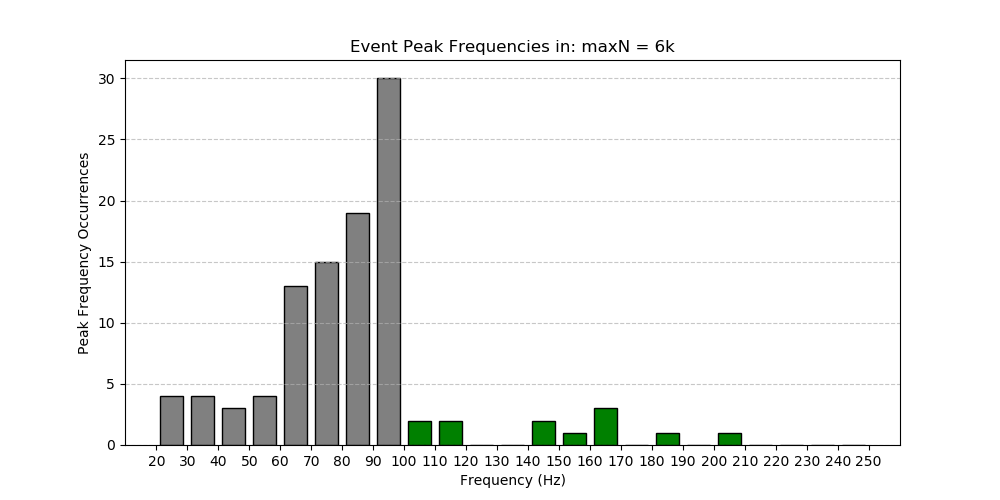
\includegraphics[width=0.75\linewidth]{images/attack_results/maxN-6k-dist.png}
            \caption{Peak frequency distribution, with a configuration of \textit{N} = 6. Showing the absolute value of event occurrences in the indicated frequency bands of 10Hz width, derived from 8 simulations of 60 seconds. Sharp wave ripple events are depicted in \textit{green}, others in \textit{grey}.}
            \label{fig:attack-neuron-6k}
        \end{figure}
        However, as figure \ref{fig:attack-neuron-6k} shows, many events fall just below the peak frequency range to qualify as SWR. This shows that this rather strong effect does to some degree depend on the exact definition of the ripple frequency range. Nonetheless, the range employed by this work is already very broad, and almost no encountered definitions, would consider lower values for ripples.\\ 
        The observed reduction of SWRs was therefore still considered to be relevant. In combination with the large increase in their duration and loss of power, the parameter certainly has a strong influence on SWRs and therefore might impair memory consolidation processes. 
        
        
        \subsubsection{Synaptic Damage (g\_max\_e)}
        Synapse damage was explored, by integrating associated reductions of synaptic conductances into the model. This was achieved by adjusting parameter \textit{g\_max\_e}, which controls the maximum conductances of all excitatory synapses in the network. Its healthy value was defined as \(60pS\) whilst the lower bound of the explored parameter range was chosen at a 20\% reduced value of \(48pS\).
        
        % Results
        \begin{figure}[htbp]
            \centering
            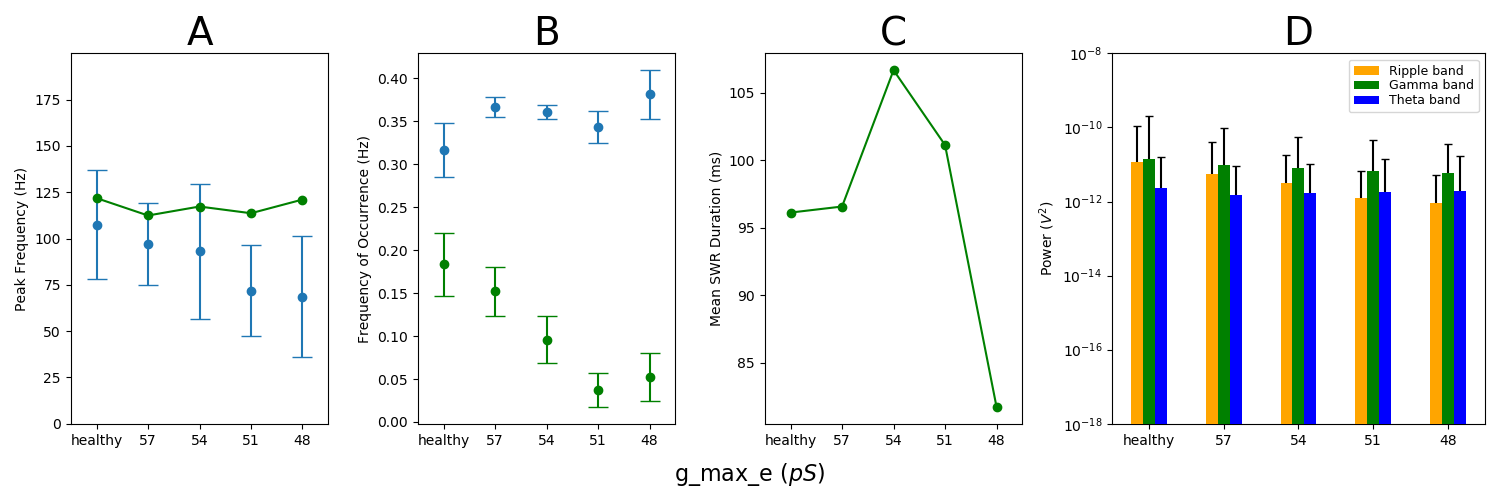
\includegraphics[width=1\linewidth]{images/attack_results/g_max_e.png}
            \caption{The impact of \textbf{g\_max\_e} on sharp wave ripples. See figure \ref{fig:attack-gCAN} for a detailed explanation. This data was derived and presented in the same fashion. Only the investigated parameters differ.}
            \label{fig:attack-g_max_e}
        \end{figure}
        The influence seems to follow the general trend of simulated attack parameters, which manifests itself as a reduction of the overall peak frequency of detected events. \textit{g\_max\_e} does however show a comparably strong influence on these event oscillations. The otherwise increasingly occurring events are therefore not qualifying as SWR. Leading to an overall reduction, that ultimately results in a SWR occurrence frequency of \textit{0.05Hz}.\\
        Besides this, \textit{g\_max\_e} shows a unique effect on the duration of events. Unlike any other analyzed parameter, it reduces the duration of SWRs. At least with the most extreme value of \textit{48pS}, a mean duration of only 82ms was observed.\\
        Whilst the decrease in sharp wave ripples already indicates a reduced memory consolidation activity, the shorter event duration can also be associated with an impairment of the process \cite{Samanta.2023}.
        
        
        \subsubsection{Overall Effect of Structural Damage}
        To assess the overall impact of structural damage on memory consolidation, the above two, individually analyzed parameters, were simultaneously adjusted. In this process, parameter values were matched that were relative to their explored ranges of similar severeness, to represent a coherent radiation state of the brain.
        
        % Results
        \begin{figure}[htbp]
            \centering
            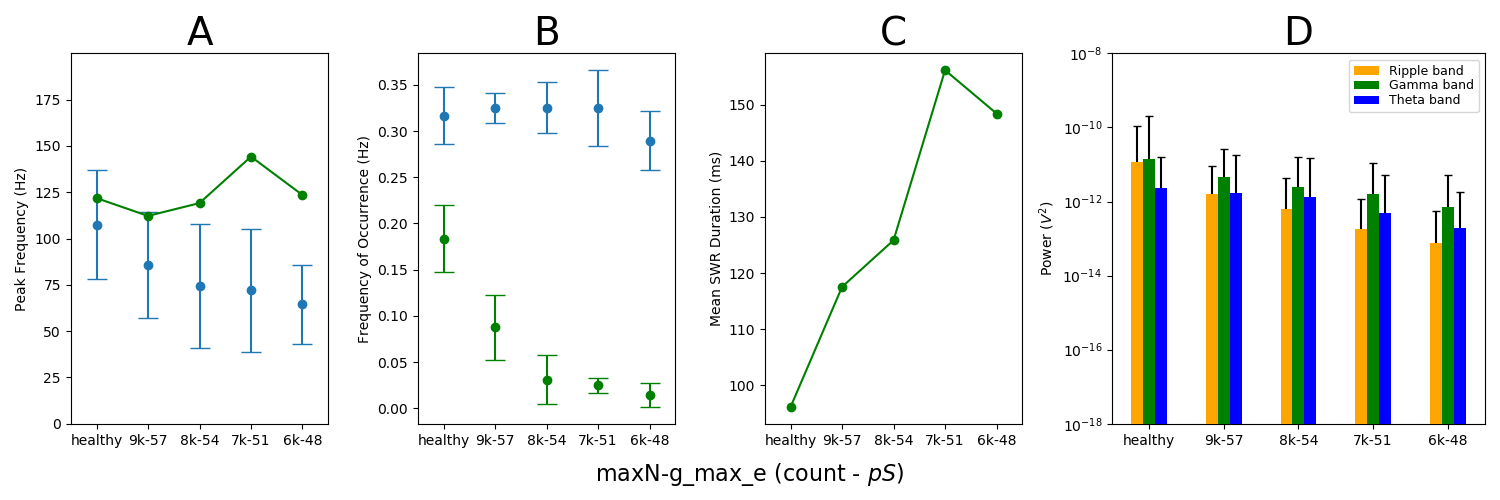
\includegraphics[width=1\linewidth]{images/attack_results/maxN-g_max_e.png}
            \caption{The overall impact of \textbf{structural damage} on sharp wave ripples. See figure \ref{fig:attack-gCAN} for a detailed explanation. This data was derived and presented in the same fashion. Only the investigated parameters differ.}
            \label{fig:attack-structural_damage}
        \end{figure}
        % Evaluation of Results
        The two included parameters produced similar results in their isolated analysis. Their combination, however, yielded results that show more extreme values, than any component. Indicating a reinforcement effect between the two.\\
        This leads to extraordinarily low values in the general peak frequencies, which are as expected, accompanied by a low number of SWRs. Whilst the SWR duration is only increased to similar levels as mentioned by \textcite{AmelieAussel.2020}, the power in all observed oscillation bands reaches relatively low values.

        Considering these observations in the context of memory consolidation, the implications are clear. With less than one sharp wave ripple occurring per minute (0.01Hz), it is to be expected that the cognitive process is impaired. Especially when also considering the other aspects. Structural damage should therefore also be considered as a potential underlying mechanism involved in the symptoms of electromagnetic attacks.


    \subsection{Full Attack}
    The following section is concerned with evaluating a \textit{full attack}, that incorporates both, neurotransmitter changes and structural damage. Like this, a more complex scenario was created, in which multiple mechanisms were employed at the same time, to represent the effects of an electromagnetic attack more realistically.\\
    To achieve this, all 4 previously presented parameters were altered simultaneously. Following the approach that was elaborated in the design section, where 4 different levels of attack intensity were explored.\\

    % Results
    \begin{figure}[htbp]
        \centering
        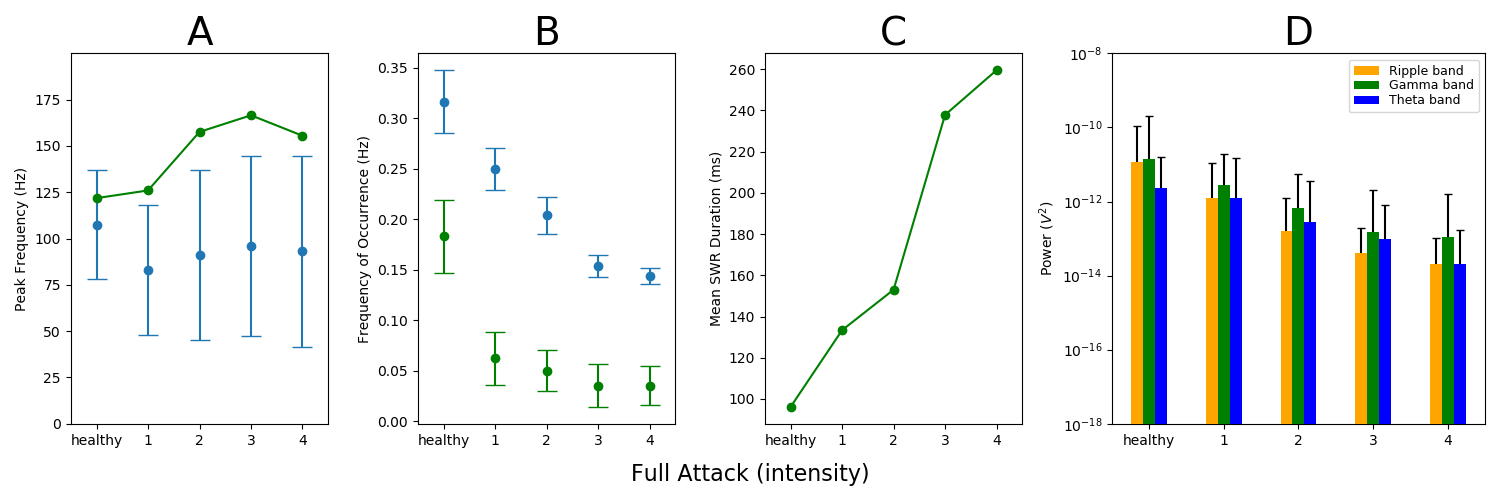
\includegraphics[width=1\linewidth]{images/attack_results/Full Attack.png}
        \caption{The impact of a \textbf{full scale attack} on sharp wave ripples. See figure \ref{fig:attack-gCAN} for a detailed explanation of the plots. This data was derived and presented in the same fashion. Parameter values at each intensity level for \textbf{(N, g\_max\_e, gCAN, gACh)} were chosen as follows: \textbf{1:} (9k-57-5-1.5), \textbf{2:} (8k-54-12-2), \textbf{3:} (7k-51-18-2.5), \textbf{4:} (6k-48-25-3).}
        \label{fig:attack-Full}
    \end{figure}
    The general result pattern does reflect the characteristics of its components. Especially considering the overall results of neurotransmitters and structural damage. Some aspects however appear only in this combined simulation.\\
    As for all attack-related results, except for those of \textit{gCAN}, the event peak frequency and occurrence of SWRs are reduced. Further indicating their connection. 
    Although the mean value of the peak frequencies does not drop far, the SWR occurrence frequency quickly reaches values around 0.05Hz. This might, however, be related to the peak frequencies' consistently large standard deviation.\\
    Most remarkable is nonetheless the SWR duration, which reaches a peak value of 238ms and thereby surpasses any reference values. But these results also incorporate the strongest decrease in power across all oscillation bands.\\

    Considering these results, a very apparent disruption of healthy SWRs can be observed. Most importantly their occurrence frequency quickly drops to about a quarter of its healthy sleep value. Suggesting that already an attack inducing the smallest intensity of alterations in the brain could disrupt memory consolidation processes. Such effects would then most likely only be reinforced with rising intensity levels since the oscillation power and SWR duration keep deviating from the healthy range.\\
    This more complex scenario could therefore already with less severe radiation exposures and resulting alterations in the brain, play a role in the learning and memory impairments of NeuroStrikes. Overall this can be considered the most robust and probable representation of an electromagnetic attack. 
    
    

% General Pattern Section beginning:
    % What was analyzed
        % Integrate in context of the work
    % How was that performed
        % keep it short and precise, no theoretical explanations
        % just motivate the approach
        % draw connection to what changes the attack configurations represent in the brain
    % Give overview of following analysis

% Subsection/Data Presentation:
    % Specifying high level meaning of parameter
        % Present parameter range
            % connect with meaning (0.5 sleep concentration, 25 waking concentration)
        % Plot
            % describe thoroughly once
            % then reference for explanation
        % discuss most relevant observations
        % relate to memory consolidation

% How could that be interpreted